\label{chapter:experiments}
\chapter{Benchmarking and Performance Regression}

By quantifying user experience, we can try to understand it better and improve it. This chapter will focus on experiments that are measuring the performance of the Tribler core, with a particular focus on user experience. Various common operations executed by users in Tribler are identified, discussed and measured.

\section{Experiments environment}
The experiments with the Tribler core are performed on a virtual private server. We tried to keep close to the specifications of a machine that an actual user could be using. The virtual server has 8GB of memory and 1 processor with 4 cores (with a clock speed of 2,5GHz). The used operation system is Ubuntu 15.10\todo{explain scenario file}. The experiments are not executed in an isolated environment but instead, in the wild, using the real Dispersy network. While these results may vary for different users, this setup can be used to derive estimations of the performance of Tribler from a user's perspective.\\\\
If not stated otherwise, the default values of the Tribler configuration file are used. These default values can be found in the `defaults.py` file in the source code directory of Tribler\footnote{https://github.com/Tribler/tribler/blob/devel/Tribler/Core/defaults.py}. All communities, except for \emph{Multichain} and \emph{BarterCast}, are loaded.\\\\
The exact steps of each experiment are specified using scenario files. In a scenario file, each line specifies a specific command of a peer at a specific time. The framework that runs these experiments, reads this file, interprets the commands to be executed and schedules them. Several constructs have been implemented to gather and write statistics to files in a processable and readable format. The usage of scenario files is already adopted in several Dispersy experiments, mainly in our \emph{AllChannel} experiment that runs on a supercomputer. We extended the usability of this approach to run a Tribler client and added various commands to support the experiments as described in this Section. The flexibility of these scenario files gives the next generation of Tribler developers a decent framework to use when doing performance analysis, scientific research and benchmarking\todo{tabel met commands?}.

\section{Profiling Tribler on low-end devices}
The addition of a REST API allows developers to have flexibility to run Tribler remotely, for instance, on embedded devices such as a Raspberry Pi. The running Tribler instance can be controlled from external devices by performing HTTP requests. Android is another example of a device that can run Tribler. During the last years, various research have been conducted to execute Tribler on Android devices\todo{cites}. Running Tribler on a low-end device, can yield much information about bottlenecks that might not be directly visible when running Tribler on a desktop or supercomputer.\\\\
The experiments described in this Section are executed on a Raspberry Pi, third generation with 1GB LPDDR2 ram, 4× ARM Cortex-A53, 1.2GHz CPU and 16GB storage on a microSD card. The used operating system is raspbian, the official system specifically designed for the Raspberry Pi, based on Debian.\\\\
Regular usage of Tribler on the Raspberry Pi using the REST API have us suspected that the Raspberry Pi is under heavy load. Monitoring the process for a while, reveals that the CPU usage is often around 100\%, completely filling up one CPU core. To get a detailed breakdown of execution time per method in the code base, the Yappi profiler has been used to analyse the performance of the Tribler session. This profiler has been integrated in the \emph{twistd} Tribler plugin and can be started together with Tribler by passing a flag when starting the plugin. The output of the profiler is a \emph{callgrind} file that can be loaded and analysed by third party software. The breakdown of a 20-minute run is visible in Figure x\todo{figure}.

\begin{figure}[!h]
	\centering
	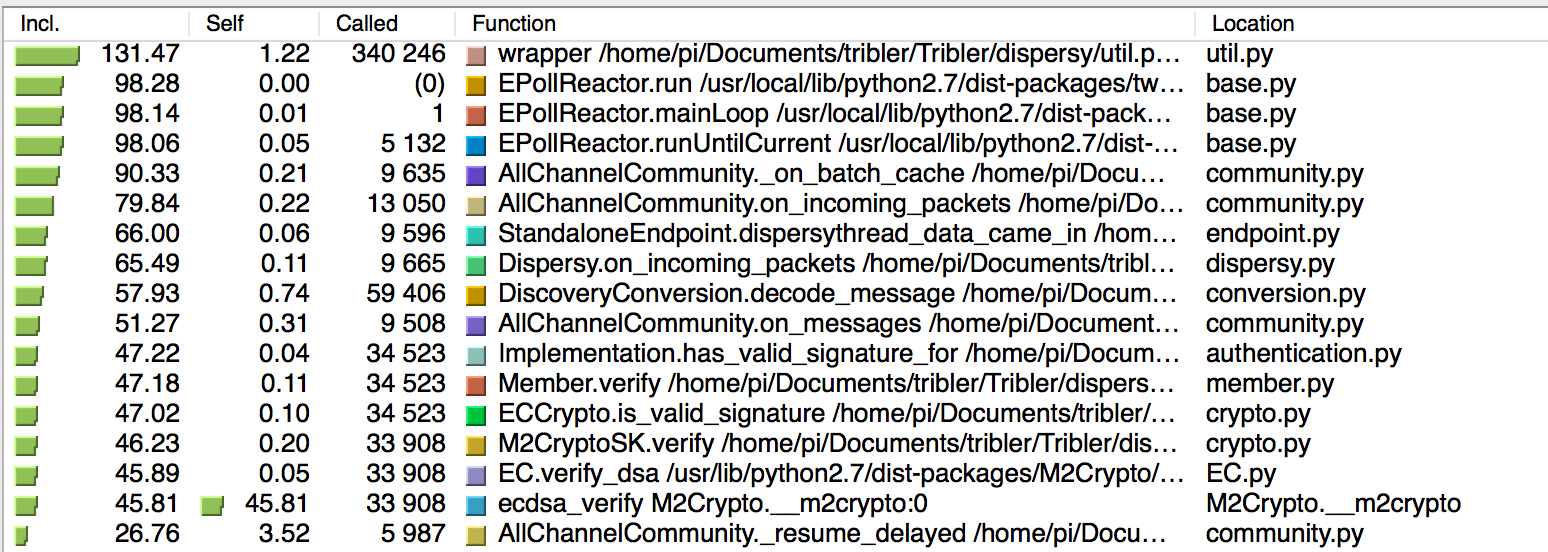
\includegraphics[width=0.9\columnwidth]{images/experiments/yappi_breakdown}
	\caption{Test.}
	\label{fig:yappi_breakdown}
\end{figure}

The file created by Yappi gives a detailed overview of the execution time of methods and can be used as a tool to detect performance bottlenecks in the system. The column \emph{Incl.} gives the inclusive cost of the function, this means the execution time of function itself and all it's including functions. The column \emph{self} gives only the execution time of the function, without considering callees. The other columns are self-explanatory and can be used to track the respective function in the source code.\\\\
From the breakdown, it is clear that Dispersy has a big impact on the performance of Tribler when running on the Raspberry Pi. The \emph{ecdsa\_verify} method is dominating the runtime of Tribler: the method is responsible for 45.81\% of the runtime. This specific method verifies the sign of an incoming Dispersy message and is invoked every time a signed message comes in. Disabling cryptographic verification of incoming messages should improve the situation, however, this is a trade-off between security and performance. By not verifying incoming messages, fake messages by an adversary can be forged and are accepted in such as system. To verify whether the responsiveness of the system improves, we measure the CPU usage of two runs. Both runs start with a non-existing Tribler state directory and have a duration of five minutes. In the first run, we are using the default configuration of Tribler, like in most of the other experiments in this Chapter. In the second run, we disable verification of incoming messages to see how things improve. The two runs are displayed in Figure \ref{fig:raspi_cpu_usage}.\\\\

\begin{figure}[!h]
	\centering
	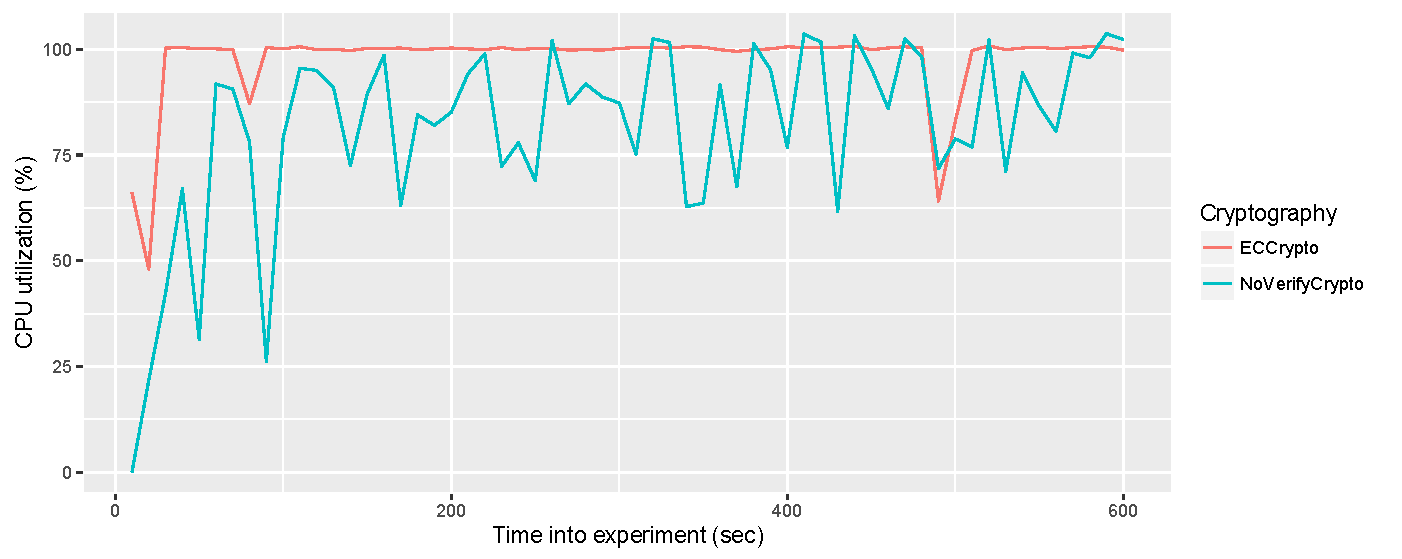
\includegraphics[width=1.0\columnwidth]{images/experiments/raspi_cpu_usage}
	\caption{Test.}
	\label{fig:raspi_cpu_usage}
\end{figure}

In the Figure, some occurrences are visible where the CPU usage appears to be over 100\%. This is explained by the fact that some of the underlying code is designed to run on multiple processors. While the threading model of Tribler is limited to a single core, the runtime and interpreter might execute code on additional cores. In the run where we enable all components of the system, the CPU usage is often 100\%. When verification of Dispersy messages is disabled, we see somewhat more drops in CPU usage but the utilization jumps back immediately to higher amounts. Disabling message verification is clearly not enough to guarantee a usable and responsive system.\\\\
To detect other performance bottlenecks, we sort the Yappi report on the \emph{Self} column to get insight in methods that are taking a long time to complete. This is visible in Figure \ref{fig:yappi_breakdown_self}. An interesting observation here is that the Python built-in \emph{all} method takes up a significant amount of time (6.13\% of the runtime). The \emph{all} method takes an iterable object and returns true if all objects of this collections are true. Both the \emph{all} method and \emph{zip} method (also visible in Figure \ref{fig:yappi_breakdown_self}) is used in the \emph{\_resume\_delayed} method. Optimization of this method is considered future work and described in GitHub issue 505\footnote{https://github.com/Tribler/dispersy/issues/505}.\\\\

\begin{figure}[!h]
	\centering
	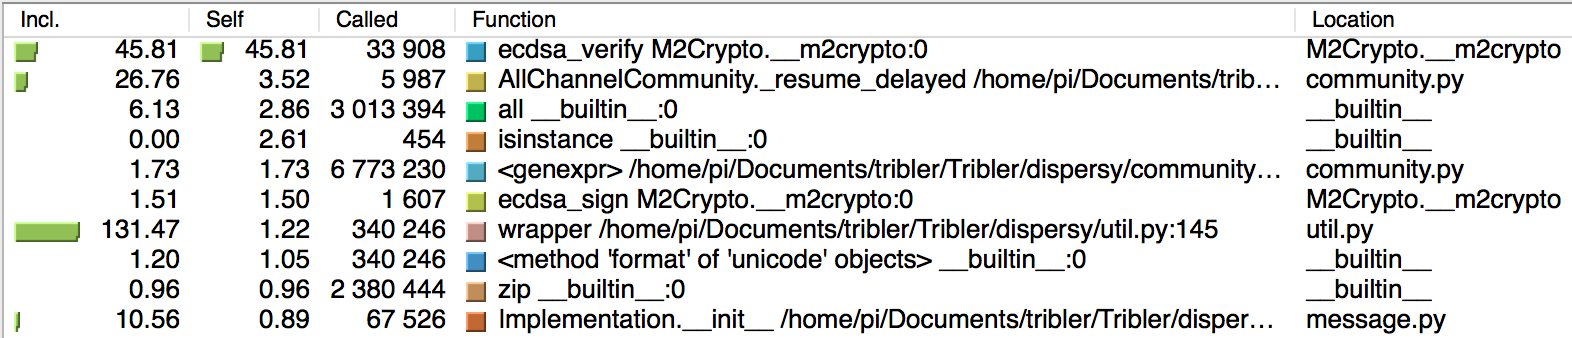
\includegraphics[width=0.9\columnwidth]{images/experiments/yappi_breakdown_self}
	\caption{Test.}
	\label{fig:yappi_breakdown_self}
\end{figure}

This shows that the Yappi profiler can be a very convenient tool to detect and track performance bottlenecks. The integration in the twistd plugin makes it easy for developers to run and analyse Tribler sessions under different circumstances.

\section{Performance of the REST API}
The performance of the REST API is directly influencing the user experience. If the response times of API calls is high, users have to wait longer before their data is available and visible. This is why we wish to make the API serve requests as fast as possible. The experiments to assess the performance of the API will particularly focus on latency of requests, however, some other statistics will be considered such as average request time, standard deviation of the response time and throughput to get more insights in the performance of the REST API.\\\\
The Apache JMeter application\cite{jmeter2010apache} is used to perform HTTP requests to Tribler and to gather and analyse performance statistics. The application allows to simulate a realistic user load, however, in this experiment we will limit the load to one user that performs a request every fixed interval. This request will be targeted to a specific endpoint in the API: \emph{/channels/discovered}. This exact call happens when users are pressing the \emph{discover} menu button in the new Qt GUI and the response of the request contains a list of all discovered that Tribler has discovered. As a consequence, the returned response can be rather large (in our experiments, the average response size is around 613KB). When the request is processed, a database lookup is performed to fetch all channels that are stored in the local database.\\\\
We perform various experiments with different intervals between requests made and a fixed amount of 500 requests. First, we perform the experiment with one request every second and we expect that the system should easily be able to hand this load and serve these requests in a timely matter. Next, the frequency of requests is increased to respectively 2, 5 and 10 requests per second. Each experiment is started around five seconds after Tribler has started where we are using a pre-filled database with around 100.000 discovered torrents and 1.200 channels. A summary of the results of these experiments are visible in Table \ref{table:performance-api-results}.\\\\

\begin{table}[]
	\centering
	\begin{tabular}{|l|l|l|l|l|l|l|}
		\hline
		\textbf{Requests/sec} & \textbf{Average (ms)} & \textbf{Std. dev (ms)} & \textbf{Median (ms)} & \textbf{Min (ms)} & \textbf{Max (ms)} & \textbf{KB/S} \\ \hline
		1 & 241 & 476.34 & 76 & 56 & 4246 & 585.58\\ \hline
		2 & 170 & 327.86 & 68 & 58 & 3394 & 1127.04\\ \hline
		5 & 123 & 210.23 & 60 & 52 & 2082 & 2538.36\\ \hline
		10 & 115 & 238.72 & 60 & 50 & 2450 & 4120.70\\ \hline
	\end{tabular}
	\caption{A summary of the experimental results when measuring the performance of the REST API.}
	\label{table:performance-api-results}
\end{table}

The most interesting observation from this table is that it appears that requests are served faster if we are performing requests at a faster rate, indicating that Tribler is able to handle the incoming requests well. This is surprising since one would expect the results to be the other way around: when the frequency of requests is increased, the average request time increases. The result is most likely due to caching of data which might be performed by the underlying database engine.\\\\
The standard deviation of the request times is rather large compared to the average request time. We think that this is due to the fact that Tribler is performing many different operations that are influencing the request times. For instance, other components of the systems such as Dispersy are performing database operations. If another process utilizes the connection to the database, the REST API might have to wait for a while before it acquires the lock, causing more request latency\todo{afmaken}.

\begin{figure}[!h]
	\centering
	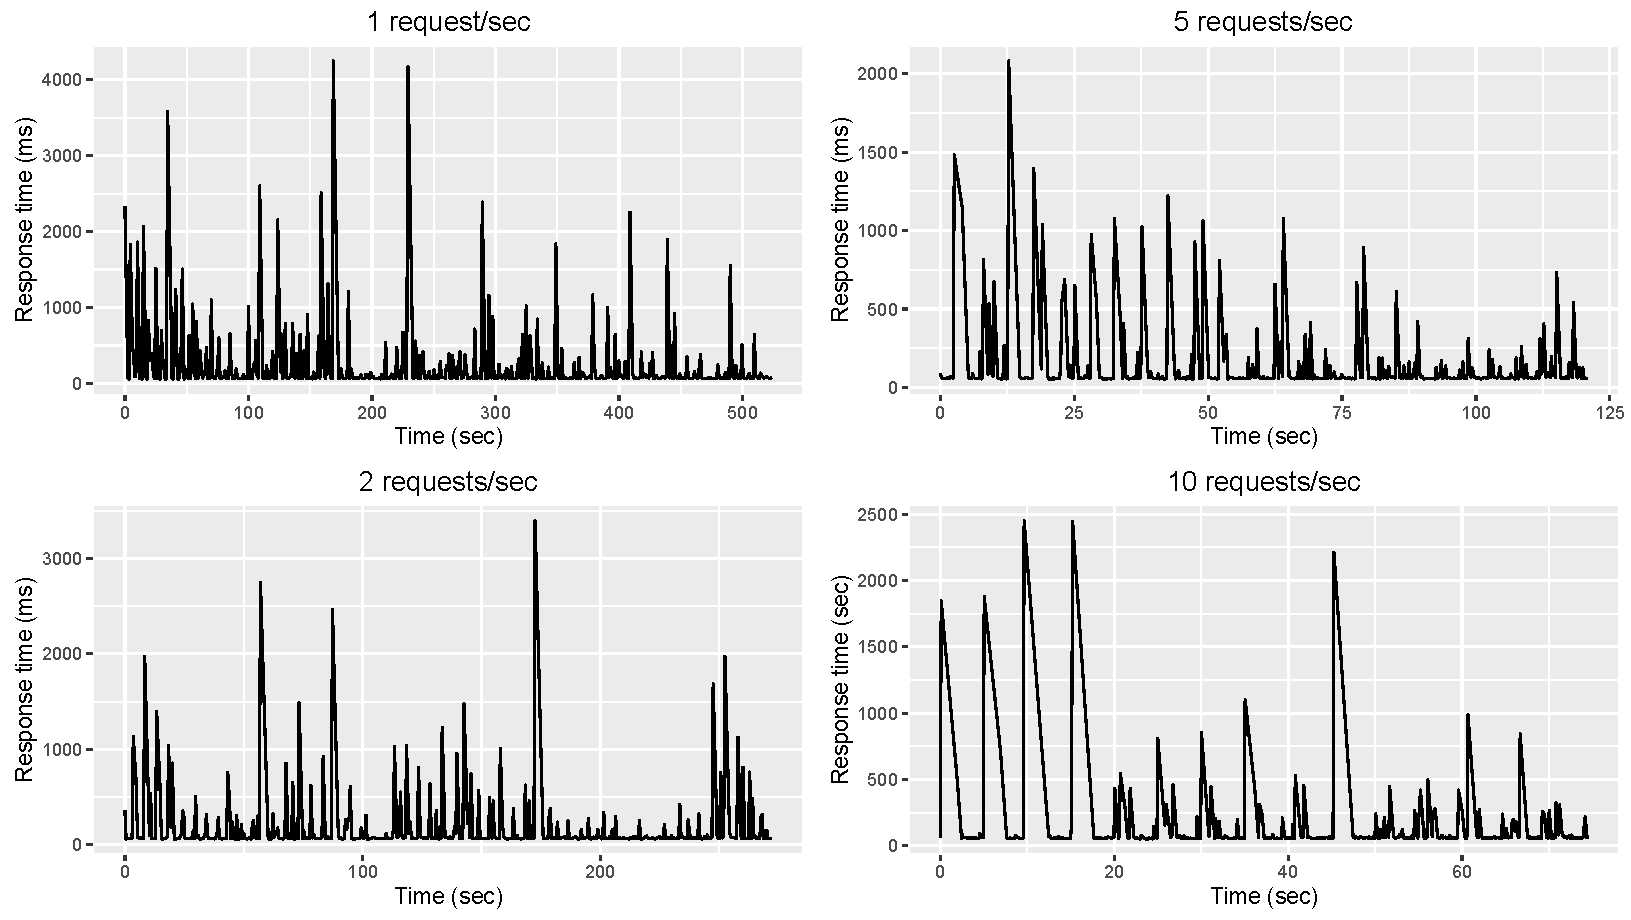
\includegraphics[width=1.0\columnwidth]{images/experiments/api_performance}
	\caption{Test.}
	\label{fig:api-performance}
\end{figure}

\begin{figure}[!h]
	\centering
	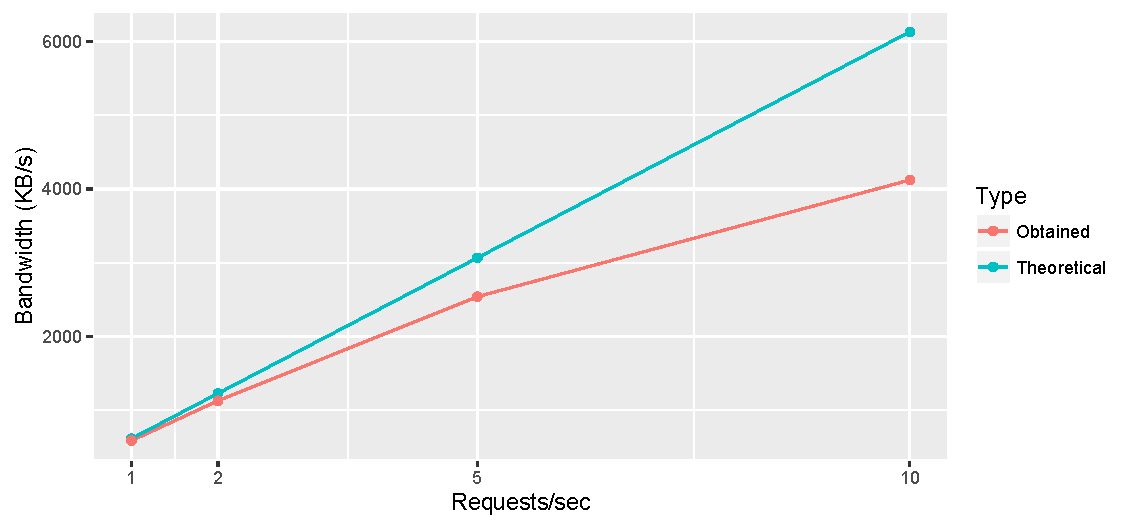
\includegraphics[width=0.8\columnwidth]{images/experiments/api_bandwidth_performance}
	\caption{The maximum theoretical bandwidth compared to the obtained bandwidth in the experiments.}
	\label{fig:api-bandwidth-performance}
\end{figure}

\section{Start-up experience}
The very first interaction that users have with Tribler, is the process of starting. During the boot process, various operations are performed:
\begin{itemize}
	\item The connection to the sqlite database is opened and initialized. If this database does not exist, it will be created.
	\item Dispersy is started and the enabled communities are loaded.
	\item Various Tribler components are created, including the video streaming server, the REST API, the remote torrent handler and the \emph{leveldb} store.
\end{itemize}
The start-up process of the Tribler core happens sequentially and no parallel operations are in place to speed up the process. Depending on the number of enabled components, the start-up time might vary.\\\\
To analyse the start-up time, Tribler is started 30 times. In half of the runs, the software is started for the first time, with no prior existing state directory. In these runs, a state directory is created and the required files are initialized. In the other half of the runs, a database with a little over 100.000 torrents is used. This database is the result of running Tribler idle for several hours, after subscribing to some popular channels. Moreover, a filled Dispersy database is used for the second half of the runs. In both scenarios, there are no downloads running. The experiment starts when the \emph{start} method of the \emph{Session} object is called and ends when the notification that Tribler has started, is observed. The results are displayed in Figure \ref{fig:startup_experiment}.\\\\
It is clear that magnitudes of the Tribler and Dispersy databases have impact on the time for Tribler to completely start. However, this impact is relatively minor since Tribler still starts within a second. We think that this statistic justifies removal of the splash screen that is shown in the old user interface. The relatively short time the splash screen would be visible in the new interface is so short that users would not even be able to read and interpret the content of the splash screen.\\\\
In both plots, some outliers are present. Further analysis learns us that these variations are caused by the loading process of the Dispersy communities, however, further investigation of the initialization part of Dispersy is considered future work.

\begin{figure}[!h]
	\centering
	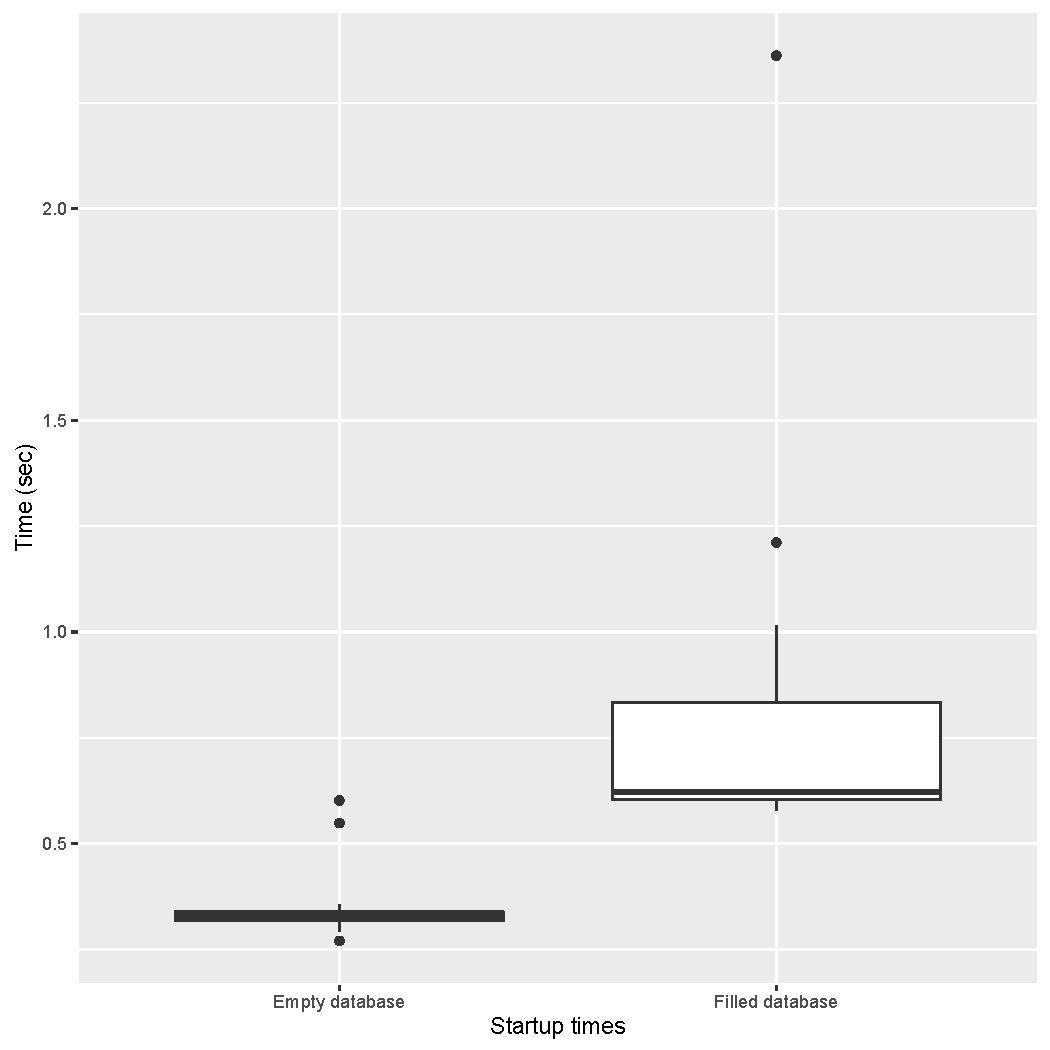
\includegraphics[width=0.6\columnwidth]{images/experiments/startup}
	\caption{Test.}
	\label{fig:startup_experiment}
\end{figure}

\section{Content Search}
We wish to serve relevant information to users as fast as possible. To help users search for relevant content, a remote keyword search has been implemented. Matching search results can either be torrents or channels. Channel results are fetched by a query in the \emph{AllChannel} community whereas torrent results are retrieved by a query in the \emph{search} community.\\\\
To verify the speed of the remote torrent search, various experiments are conducted. We are using a list of 100 terms that users might be searching for. This list of search terms can be found in Appendix x\todo{Add this}. Each query is executed when there are at least 20 connected peers in the \emph{SearchCommunity}. The timeout period of the remote search is 60 seconds. This experiment has a particular focus on two statistics: the time until the first remote torrent search results comes in and the turnaround time of the search request. We should note that users performing a remote search might see results earlier since in parallel, a  search query in the local database is performed. The results are visible in Figure \ref{fig:remote_search_first_result} and \ref{fig:remote_search_all_result}.\todo{nitin graph}\\\\
Overall, the remote torrent search as implemented in Tribler is very fast and performs well. On average, 61 search results are returned for each query and the first incoming torrent result takes 0.26 seconds to arrive. As we see in Figure \ref{fig:remote_search_first_result}, over 90\% of the first remote search results are available to the user within a second. During our experiment, we always have the first incoming torrent result within 3.5 seconds.\\\\
The other graphs shows the turnaround time of the request. On average, it takes 2.1 seconds for all torrent search results to arrive. From Figure \ref{fig:remote_search_all_result}, we see that in over 90\% of the search queries, we have all results within 10 seconds.

\begin{figure}[!h]
	\centering
	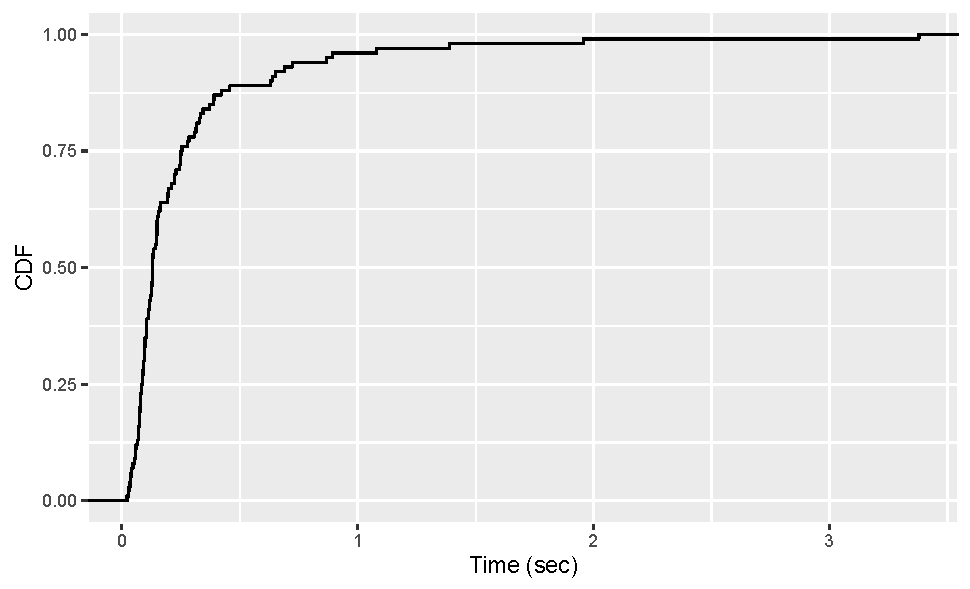
\includegraphics[width=0.6\columnwidth]{images/experiments/cdf_remote_search_first_results}
	\caption{Test.}
	\label{fig:remote_search_first_result}
\end{figure}

\begin{figure}[!h]
	\centering
	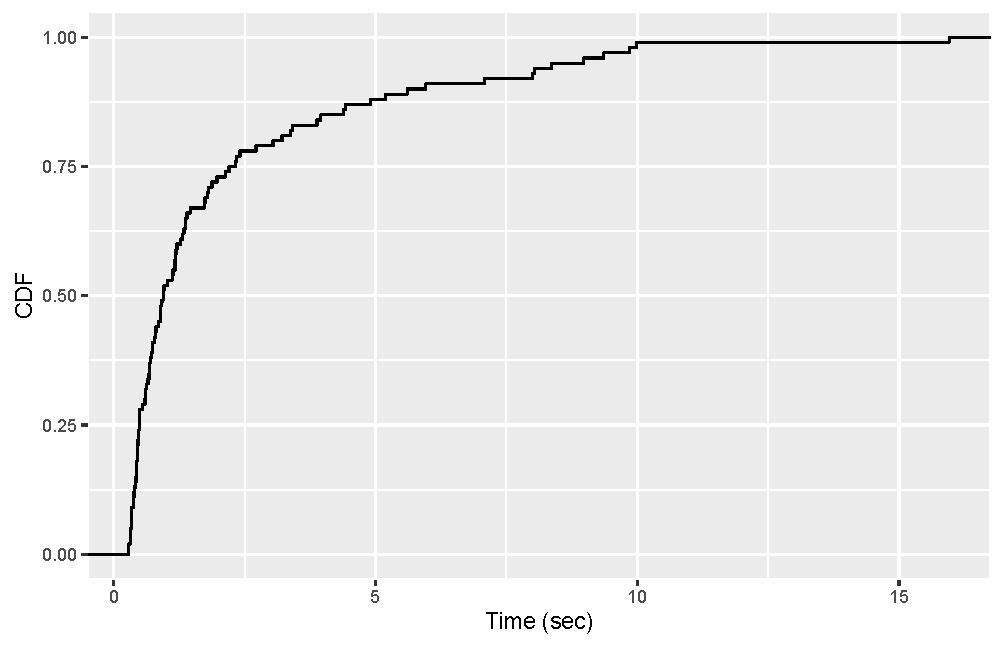
\includegraphics[width=0.6\columnwidth]{images/experiments/cdf_remote_search_all_results}
	\caption{Test.}
	\label{fig:remote_search_all_result}
\end{figure}

\section{Local keyword search}
...

\section{Video streaming}
The embedded video player in Tribler allows users to watch a video that is being downloaded. Available since Tribler 4.0, the video playback did not evolve much. The video player is based on VLC and offers support for seeking so the user can jump randomly to a specified offset in the video. Video downloads have a special Video On Demand (VOD) mode which means that the libtorrent library piece picking mechanism uses a linear policy. In this mode, pieces are downloaded in a timely matter. When the user seeks to a position in the video, the prioritization of the pieces are modified, giving priority to pieces around the chosen seek position. Users also have the possibility to use an external video player that support playback of HTTP video streams.\\\\
The bytes are streamed to a VLC client using HTTP. When Tribler starts, a HTTP video server is started. This server supports HTTP range requests which means that a specific part of a video file can be queried by using the HTTP \emph{range} header. This is useful when the user performs a seeking operation since only a specific part of the file has to be returned in the HTTP response. If some pieces are not available, the video server will wait until these bytes are downloaded and available before returning these bytes in the response.\\\\
To improve user experience, we wish to minimize the delay that users experience when performing a seek operation in the video player. The experiment performed in this Section, will measure the buffering delay. For this purpose, the well-seeded \emph{Big Buck Bunny}\footnote{https://peach.blender.org} movie will be downloaded. We will perform various HTTP range requests using the \emph{curl} command line tool. Every request, 10 megabyte of data will be requested and we will measure the total request time for each of these requests. The results are visible Table \ref{table:video_player_seek_times}.\\

\begin{table}[]
	\centering
	\label{table:video_player_seek_times}
	\begin{tabular}{|l|l|}
		\hline
		First byte               & Request time (sec) \\ \hline
		0                        & 11.6                  \\ \hline
		$ 1 * 10^9 $ & 64.4                  \\ \hline
		$ 2 * 10^9 $ & 64.6                  \\ \hline
		$ 3 * 10^9 $ & 65.9                   \\ \hline
		$ 4 * 10^9 $ & 100.6                   \\ \hline
		$ 5 * 10^9 $ & 115.6                   \\ \hline
		$ 6 * 10^9 $ & 115.8                  \\ \hline
		$ 7 * 10^9 $ & 12.2                  \\ \hline
		$ 8 * 10^9 $ & 66.6                   \\ \hline
		$ 9 * 10^9 $ & 52.4                   \\ \hline
	\end{tabular}
	\caption{My caption}
\end{table}

Theoretically, we would expect around the same request time for each range request, assuming that the availability of each piece is high. When performing a seek, the piece picking mechanism adjusts priorities and these prioritized pieces should start to download immediately. The experiments shows some serious flaws in this mechanism where it might take up to two minutes for data to be available. Further investigation of this issue learns us that the video player always tries to download the first 10\% of the video file, except the 7th run of the experiment, where the prioritizing seems to be correctly applied. Solving this bug is considered further work and described in more detail on Github issue 1234\todo{issue maken}.

\section{Content discovery}
Content discovery is one of the most important features of Tribler. By running Tribler idle for a while, content is synchronized with other peers using the Dispersy framework. When a user starts Tribler for the first time, there is no available content yet. In this Section, we will verify the content discovery speed after the first start. The experiment is structured as follows: we measure the interval from the completion of start procedure to the moment where the first content is discovered. This is done for both torrents and channels and repeated 15 times. The results of this experiment are visible in Figure \ref{fig:content_discovery_speed}.

\begin{figure}[!h]
	\centering
	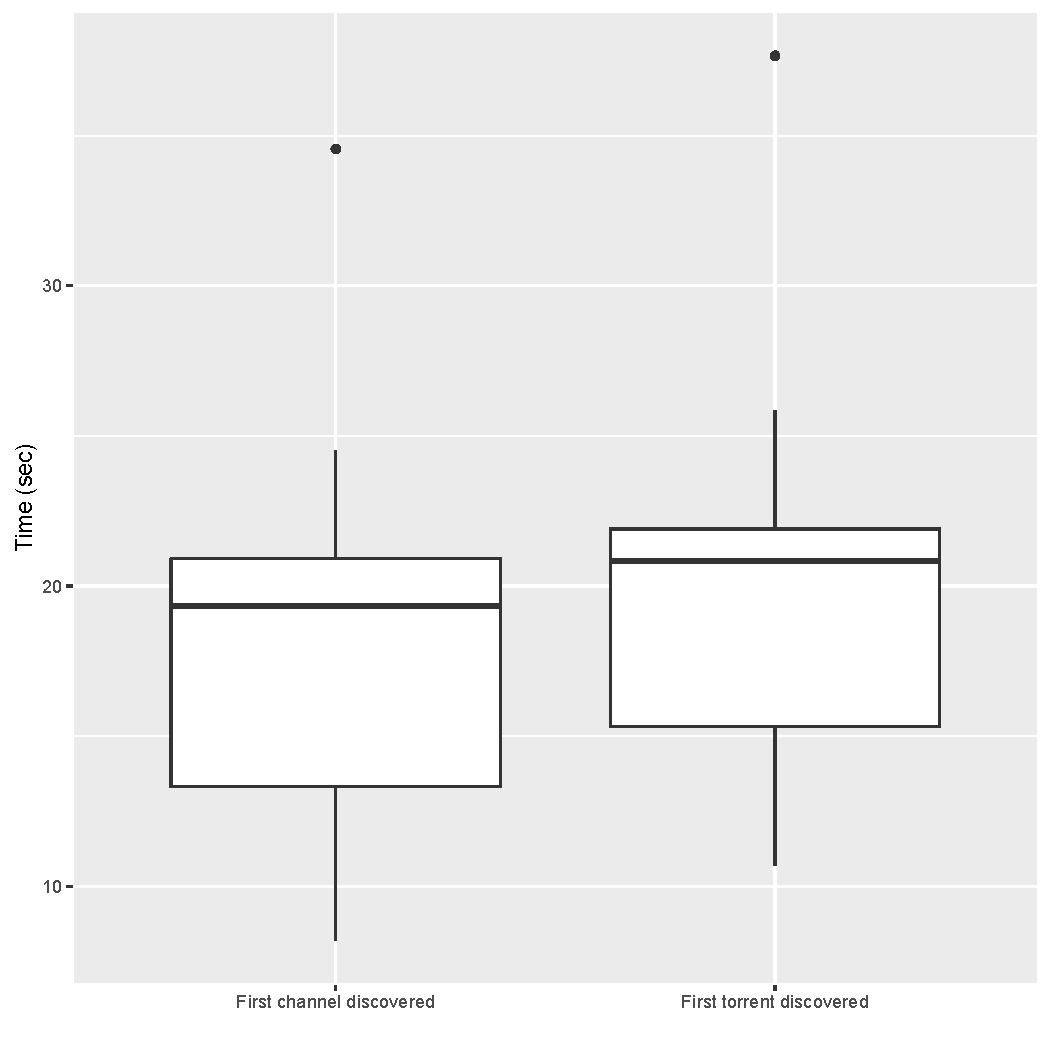
\includegraphics[width=0.6\columnwidth]{images/experiments/content_discovery_speed}
	\caption{Test.}
	\label{fig:content_discovery_speed}
\end{figure}

The delay of discovering the first channel is reasonably. In all runs, we have our first content available within 35 seconds. Discovery times of the first torrent is slightly slower and in all runs, the first torrent in a channel is discovered within 40 seconds. In the old user interface, users were presented with a blank screen with no feedback about new discovered content. In the new interface, the user is presented with a screen that informs the user that Tribler is discovering the first content. This screen is only shown the first time Tribler is started.

\section{Channel subscription}
When Tribler runs idle, not all content is discovered. The majority of content is discovered when users are subscribing to channel. When Tribler discovers a channel, users are presented with a preview of this channel. Internally, Tribler joins a \emph{PreviewChannelCommunity}, a community derived from the main \emph{ChannelCommunity}. I this preview, the amount of torrents to be collected is limited. The associated \emph{ChannelCommunity} is joined the moment the user subscribes to a channel, after which the full range of content is synchronized with the subscribed user. Removing the preview mechanism significantly increases the resource usage of the Tribler session since the amount of incoming messages to be decoded and verified will rise.\\\\
The experiment as described in this Section, will focus on the discovery speed of additional content after the user subscribes to a specific channel. For this experiment, the 20 most popular channels (with the most subscribers) are determined. A Tribler state directory has been installed that discovered channels but did not subscribe to any of them. Exactly 10 seconds after Tribler started, we subscribe to one of these channels and we measure the interval between subscriptions and discovery of the first additional torrent in this channel. Tribler is restarted between every run so we guarantee a clean state of the system. The results are visible in Figure \ref{fig:channel_subscription}.

\begin{figure}[!h]
	\centering
	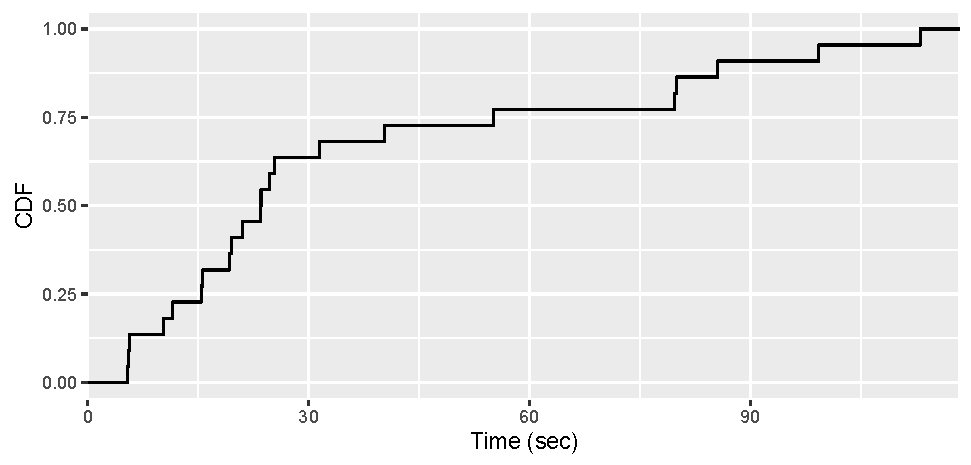
\includegraphics[width=0.9\columnwidth]{images/experiments/channel_subscription}
	\caption{Test.}
	\label{fig:channel_subscription}
\end{figure}

The average discovery time of additional torrents is 36.8 seconds, which is quite long, compared to the performance of remote search. The discovery times have a somehow high variation as can be seen in Figure \ref{fig:channel_subscription}. This can be explained by the fact that immediately after subscribing to a channel, new peers have to be found in the \emph{ChannelCommunity} that is joined after subscription. Moreover, some of the channels might have more torrents available. After subscription to a channel with a higher amount of torrents, it is more likely for content to be discovered faster.\\\\
To verify the impact of automatically subscribing to each channel, we perform a CPU usage measurement. In two idle runs of a Tribler sessions, both lasting for ten minutes, we measure the CPU usage every ten seconds. In the first run, a regular Tribler session is used where previews of discovered channels are enabled. In the second run, we bypass the preview of a discovered channel and immediately join the channel, synchronizing all available content. The results of this experiment are visible in Figure \ref{fig:channel_subscription_cpu}.

\begin{figure}[!h]
	\centering
	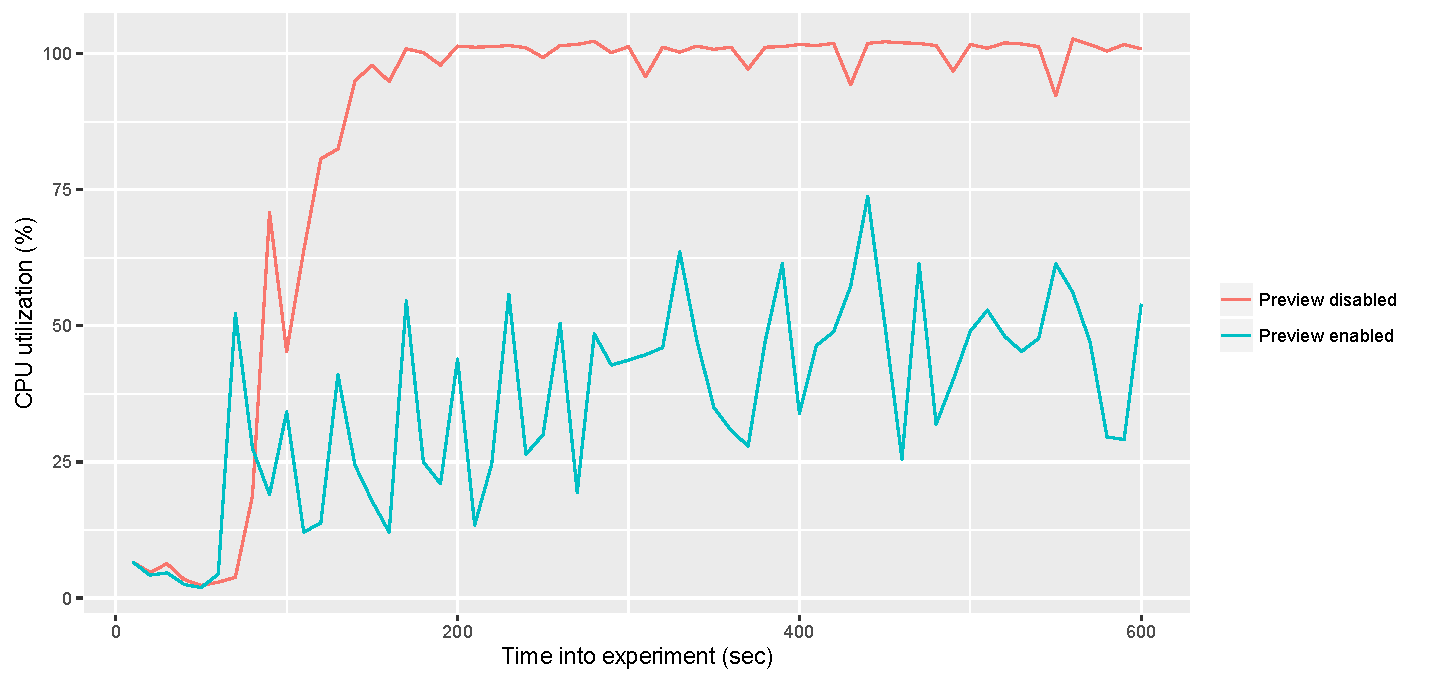
\includegraphics[width=1.0\columnwidth]{images/experiments/subscribe_cpu_experiment}
	\caption{Test.}
	\label{fig:channel_subscription_cpu}
\end{figure}

Whereas the CPU usage of the normal run is around 50\% on average, the CPU is busy when we enable auto-join of channels. This shows that it is infeasible to enable this auto-join feature. One might limit the number of fetched torrents, however, this requires a feedback mechanism where we should notify other peers to limit the amount of messages sent to the peer that is discovering content in the channel. Implementing of such as feature is considered future work.

\section{Torrent Availability and Lookup Performance}
A possible source of torrents is the Distributed Hash Table (DHT). The DHT provides primitives to query torrent files and peers, based on a specific infohash of a torrent. Querying the DHT for torrent files can be done by invoking the \emph{download\_torrentfile} in the \emph{Session} object. One should specify the callback to be invoked after the metainfo is successfully downloaded. In this Section, experiments will be conducted to get insights in the availability of torrent files and the performance of lookup operations in the DHT. This experiment is relevant since users that want to determine whether specific content is interesting or not, first might want to view metainfo of the torrent file. This metainfo should be available as soon as possible.\\\\
In the current user interface, the torrent file is fetched when the user single clicks on a torrent in the list of torrents, either when browsing through contents of a channel or after performing a remote keyword search. In addition, when executing a remote search, the first three top-results are pre-fetched since the user might be interested in them. For this experiment, a popular channel with over 5.000 torrents is taken and a subset of infohashes of torrents in this channel is calculated. Every 40 seconds, a DHT query is performed with one of the 1.000 random infohashes. The timeout period used in Tribler is 30 seconds, after which a failure callback is invoked and an error is displayed in the user interface. The results of this experiments are visible in Figure \ref{fig:metainfo_fetch}. Torrents that cannot be successfully resolved from the DHT, are assigned a value of 30 seconds in the graph.\\\\

\begin{figure}[!h]
	\centering
	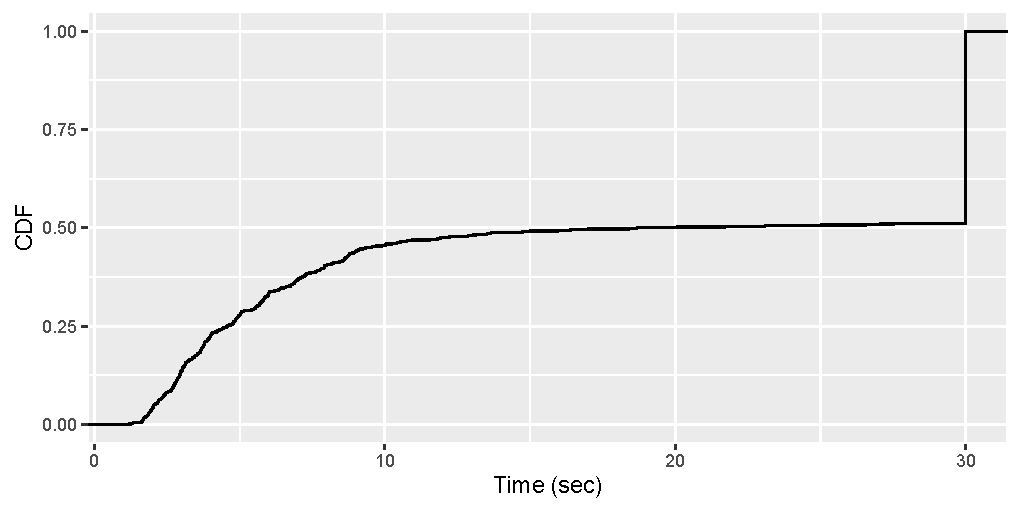
\includegraphics[width=0.9\columnwidth]{images/experiments/metainfo_fetch}
	\caption{Test.}
	\label{fig:metainfo_fetch}
\end{figure}

We immediately notice that the failure rate of DHT lookups is quite high: a little under 50\% of the lookup operations are timing out. This might be addressed to dead torrents (no peers in the DHT have this torrent available) or private torrents (torrents which information is not spread in the DHT). The amount of failures might be even higher in a less popular channel since the content in these channels are less seeded. We should note that the DHT is not the only source of torrents in Tribler. When performing a remote query search, each incoming torrent result might have candidates attached that possibly have this torrent in their database. When clicking on a torrent result in the list of search results, not only the DHT is queried, each of the candidates of the torrent result is queried in parallel using the Trivial File Transfer Protocol (TFTP)\cite{sollins1992tftp}. TFTP is a simplified version of the more sophisticated File Transfer Protocol which is commonly used to transfer files between web servers. Tribler contains a dedicated Python package with a TFTP implementation. Unfortunately, the approach of fetching metainfo of torrents from other peers is only usable when searching for torrents. Caching and exchanging torrent candidates is not successful since the availability of candidates later cannot be guaranteed.\\\\
The average lookup time of torrents that are successfully fetched from the DHT is 5.81 seconds which is reasonably fast. Additionally, Figure \ref{fig:metainfo_fetch} shows that a little over 90\% of the successfully fetched torrents are retrieved within 10 seconds.\\\\
To improve performance of metainfo lookup, dead torrents should be handled correctly. One possible solution might be an implementation of a periodical check for each incoming torrent. By limiting the number of outstanding DHT requests, this approach does not create require much additional resources. To further improve performance, the result of DHT lookups might be disseminated to remote peers in the network. Torrents that are not successfully fetched from the DHT, could be hidden automatically in the user interface. The downside of this approach is that it might not give a realistic view of the availability of a torrent since their might be candidates which have a copy of this torrent available.